\documentclass[a4paper,12pt]{article}

\usepackage[T1]{fontenc}
\usepackage[utf8]{inputenc}
\usepackage[francais]{babel}
\usepackage{multirow,array}
\usepackage{graphicx}
\usepackage{a4wide}
\newcommand{\HRule}{\rule{\linewidth}{1mm}}

\begin{document}


%
%  TITEL
%

\begin{titlepage}

\begin{center}
\huge Fast spatial localization \\ with an octree structure
\HRule \\
\medskip
{\Huge \bfseries The libOL library} \\
\HRule
\end{center}

\vspace*{\stretch{3}}

\begin{figure}[htbp]
\begin{center}
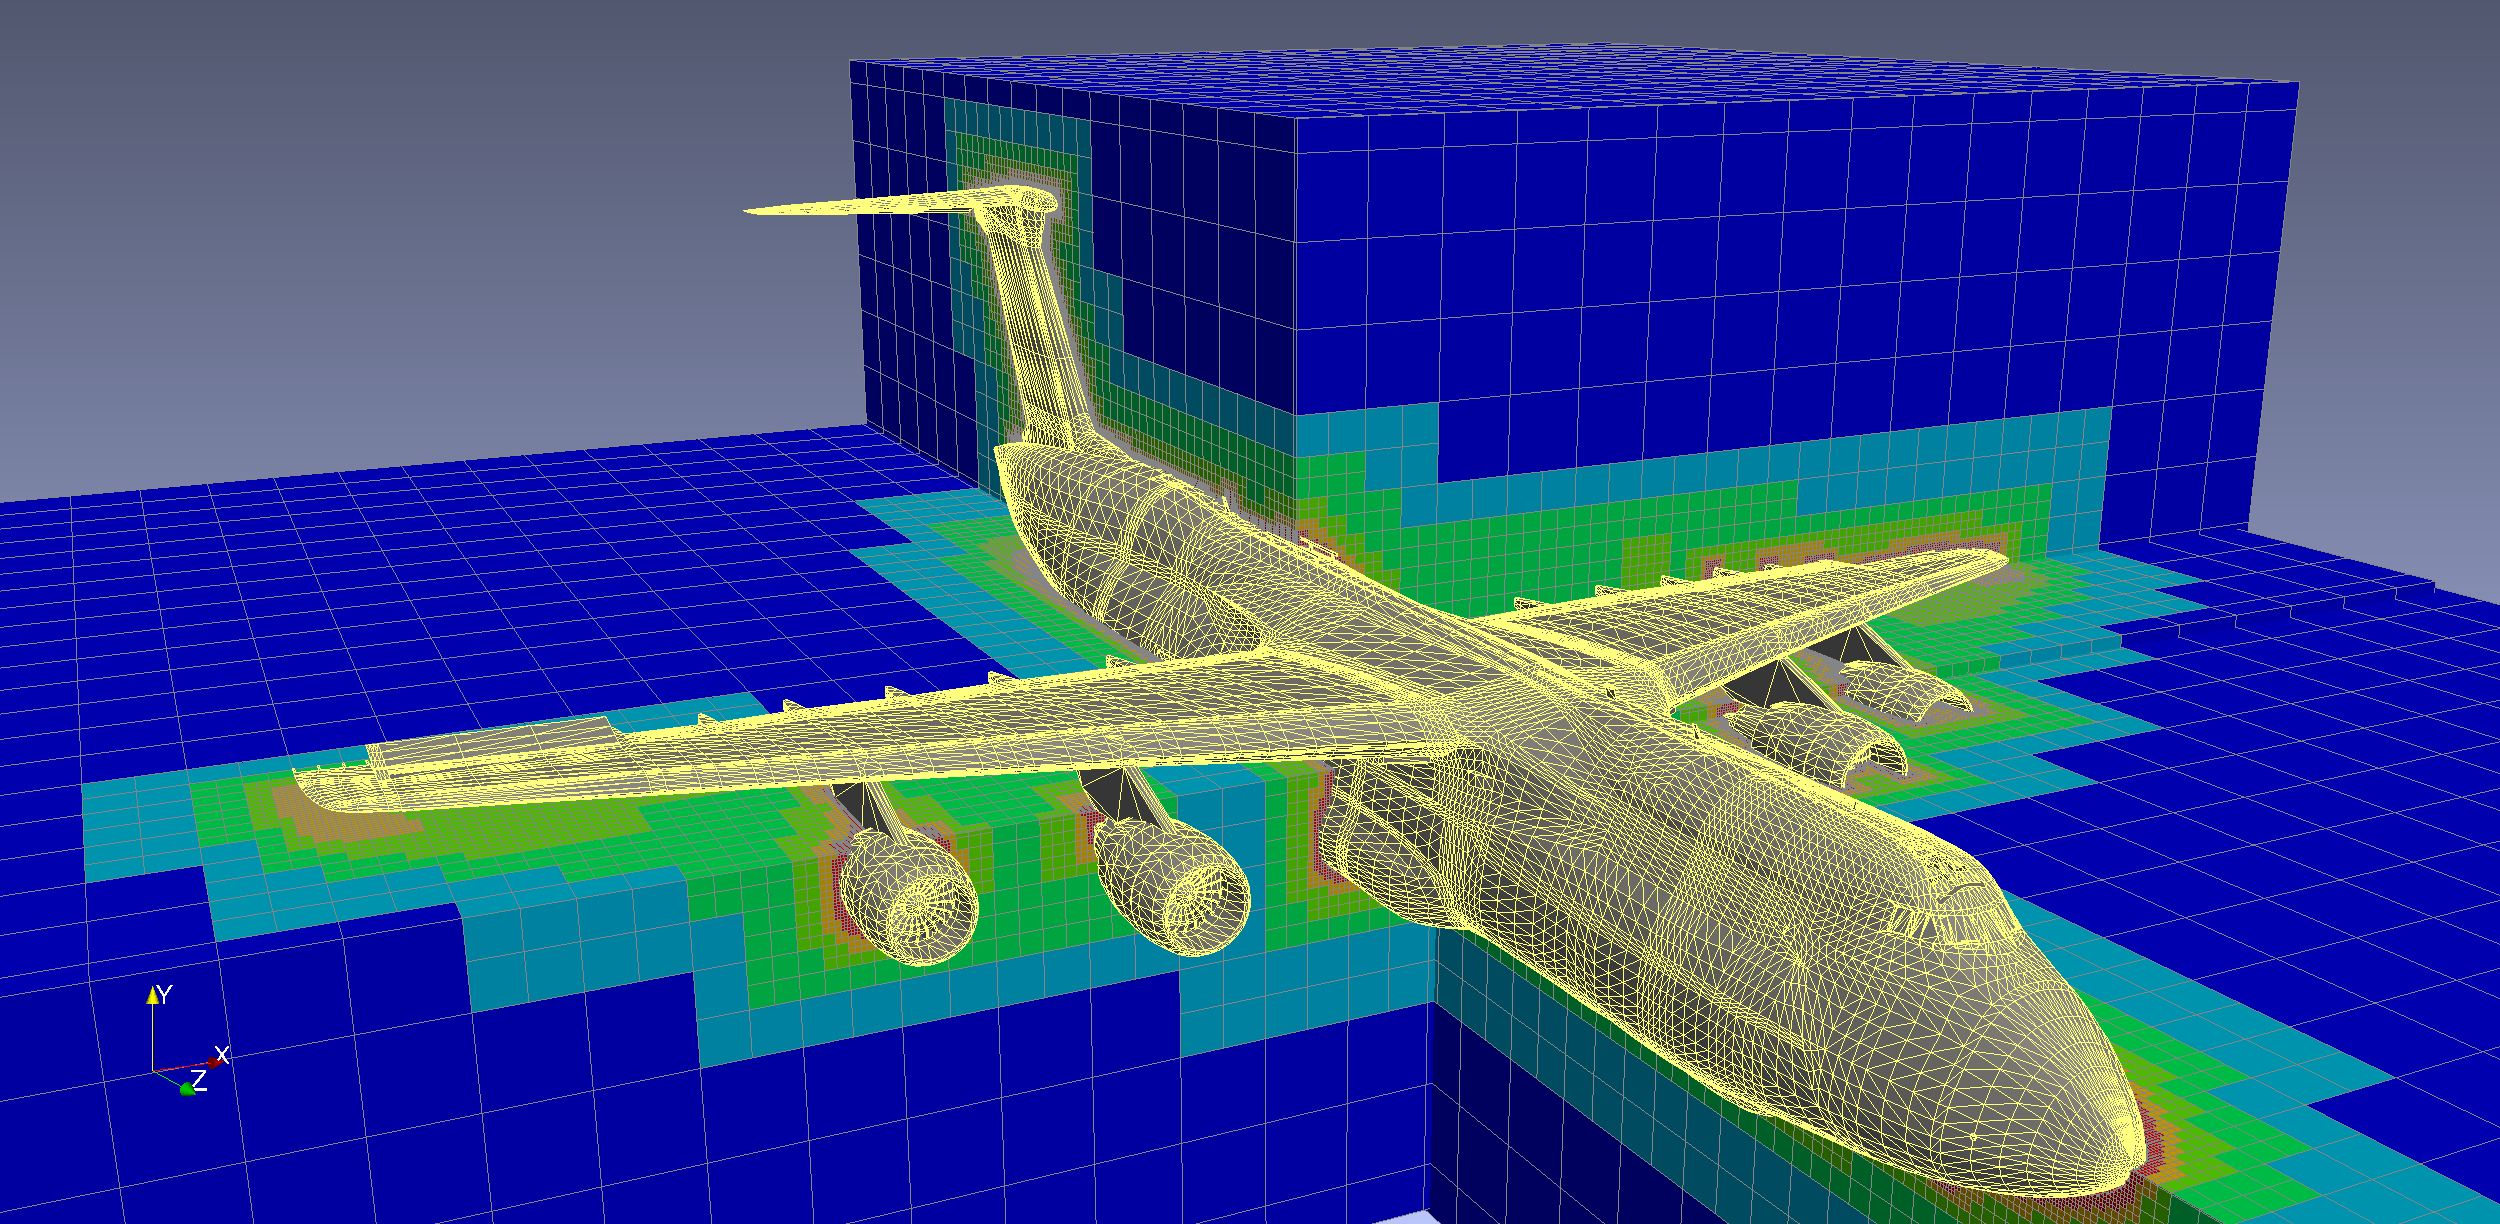
\includegraphics[height=7.8cm]{octree_mesh.png}
\end{center}
\end{figure}

\vspace*{\stretch{1}}

\begin{flushright}
\Large Lo\"ic MAR\'ECHAL / INRIA, Gamma project\\
\Large February 2021 \\
\normalsize Document v1.50, library v1.70
\end{flushright}

\end{titlepage}

\clearpage

\setcounter{tocdepth}{2}
\renewcommand*\contentsname{Table of contents}
\tableofcontents
\vfill

\footnotesize{Cover picture: octree structure of a Lockheed C-5 Galaxy made by Thomas Døhlen.}
\normalsize

\clearpage


%
%  1 / INTRODUCTION
%

\section{Introduction}
The libOL's purpose is to facilitate the spatial localization of mesh entities by allowing basic geometrical queries like searching the closest triangle from a point or building the list of tetrahedra intersected by a bounding rectangle.

The octree build is fast and straightforward and handles many different kinds of mesh entities such as vertices, edges, triangles, quadrilaterals and tetrahedra. The queries can be controlled by specifying the kind of element to look for, the maximum search distance and filtered through a user-defined function.

Two of its main key points are its very small memory footprint, on the order of 10 GB per billion elements, and fast execution time, thanks to the library being thread-safe, make it possible to make queries concurrently.


%
%  2 / USAGE
%

\section{Usage}
The input data needed by the library is a mesh in its most basic form: a table of nodes coordinates and some optional elements' connectivity. The libOL generates an octree from this mesh so that its octants, the basic cubic octree's element, contains no more than 20 mesh entities in order to speedup calculation. Consequently, the time and memory needed to build the octree are dependent of the mesh size but also of its geometrical shape. Indeed, as an octree structure is isotropic, very thin or sharp geometries will need more octants to capture those fine features, thus increasing the machine resources needed.

A libOL octree structure can contain only one mesh, so there may be only one table for each kind of data (you cannot have two triangle tables, one for boundary elements and the other one for internal triangles between each pair of tetrahedra). However, you may allocate several octree structures, each defined by its own unique tag, so that each could store a triangle table that may relate to the same mesh.

Let's say that we have a mesh made of $NmbVer$ vertices stored in the table $VerCrd$ and $NmbTri[]$ triangles stored in the table $TriTab[]$ and we wish to look for the closest triangle from the point of coordinates $\{0.5, 2.3, -6.0\}$ as well as the list of triangles included in the rectangular area centered in $\{2,2,10\}$ and diameter $2$. Here is the simplified source code:

\begin{tt}
\begin{verbatim}
int64_t OctIdx;
int IntersectedTriangles[10];
int NmbVer, NmbTri, (*TriTab)[3];
double (*CrdTab)[3], VerCrd[3]={0.5, 2.3, -6.0};
double BoxMin[3]={1,1,9}, BoxMax[3]={3,3,11}, MinDis;
...
(your mesh allocation and reading)
...
OctIdx = LolNewOctree(
         NmbVer, VerTab[1], VerTab[2],
              0,      NULL,      NULL,
         NmbTri, TriTab[1], TriTab[1],
              0,      NULL,      NULL,
              0,      NULL,      NULL,
              0,      NULL,      NULL,
              0,      NULL,      NULL,
              0,      NULL,      NULL,
              1, 1);

printf("Octree number %d has been build\n", OctIdx);

TriIdx = LolGetNearest(OctIdx, TypTri, VerCrd, &MinDis, 0, NULL, NULL, 0);
printf("the closest triangle from 0.5, 2.3, -6.0 is: %d\n", TriIdx);

NmbBoxTri = LolGetBoundingBox(OctIdx, TypTri, 10, TriTab, BoxMin, BoxMax, 0);
for(i=0;i<NmbTri;i++)
    printf("triangle number: %d\n", TriTab[i]);

LolFreeOctree(OctIdx);
\end{verbatim}
\end{tt}
\normalfont


%
%  3 / COMMANDS
%

\clearpage
\section{List of commands}


\subsection{LolFreeOctree}
Simply free an octree structure with all related data and return the total memory used by thie instance.
The function does not terminate the library and further octrees can be allocated.

\subsubsection*{Syntax}
{\tt mem = LolFreeOctree(OctIdx);}


\subsection{LolGetBoundingBox}
Intersect the whole mesh with a rectangular box and return the list of entities included in this area.
The intersection test is restricted to a single kind of entity and can be performed concurrently as long as the calling processes provide a unique index. The list of entities is stored in a user-provided table whose size must be given and will limit the number of returned included elements.

\subsubsection*{Syntax}
\begin{tt}
\begin{verbatim}
NmbTri = LolGetBoundingBox(
         OctIdx, typ, MaxTri, TriTab,
         BoxMin[3], BoxMax[3], ThrIdx);
\end{verbatim}
\end{tt}
\normalfont

\subsubsection*{Parameters}
\begin{tabular}{|m{3cm}|m{2cm}|m{8.5cm}|}
\hline
Parameter  & type      & description \\
\hline
OctIdx     & int64\_t  & octree index as returned by LolNewOctree() \\
\hline
typ        & int       & kind of mesh entity to look for: LolTypVer, LolTypEdg, LolTypTri, LolTypQad or LolTypTet \\
\hline
MaxTri     & int       & size of the user-provided elements table \\
\hline
TriTab     & int *     & pointer to a user-provided table that will be filled with the intersected elements \\
\hline
BoxMin     & double [3] & coordinates of the upper bounding box corner \\
\hline
BoxMin     & double [3] & coordinates of the lower bounding box corner \\
\hline
ThrIdx     & int        & thread or calling process number or 0 in serial case \\
\hline
\end{tabular}

\medskip

\begin{tabular}{|m{3cm}|m{2cm}|m{8.5cm}|}
\hline
Return     & type   & description \\
\hline
index      & int    & return the number of entities included in the box \\
\hline
\end{tabular}

\subsubsection*{Example}
Allocate a return table with 10 entries and ask for the libOL to find the first 10 triangles intersected by the box $\{0,0,0\} - \{1,1,1\}$ and print their indices.

\begin{tt}
\begin{verbatim}
int TriTab[10];
double box[2][3]={{0,0,0}, {1,1,1}};
NmbTri = LolGetBoundingBox(OctIdx, TypTri, 10, TriTab, box[0], box[1], 0);
for(i=0;i<NmbTri;i++)
    printf("triangle numéro : %d\n", TriTab[i]);
\end{verbatim}
\end{tt}
\normalfont


\subsection{LolGetNearest}
Search for the closest mesh entity from a given point. The kind of entity to search for can be restricted to a specified type or filtered through a user function (see the comment section in LolIntersectSurface for more information) or to a maximum distance from the source point. This procedure can safely be called in parallel as long as the concurrent caller's ID are unique.

\subsubsection*{Syntax}
\begin{tt}
\begin{verbatim}
index = LolGetNearest(
        OctIdx, typ, crd, PtrMinDis, MaxDis,
        UsrPrc, UsrDat, ThrIdx);
\end{verbatim}
\end{tt}
\normalfont

\subsubsection*{Parameters}
\begin{tabular}{|m{3cm}|m{2cm}|m{8.5cm}|}
\hline
Parameter  & type       & description \\
\hline
OctIdx     & int64\_t   & octree index as returned by LolNewOctree() \\
\hline
typ        & int        & kind of entity to look for: LolTypVer, LolTypEdg, LolTypTri, LolTypQad or LolTypTet \\
\hline
crd        & double [3] & coordinates of the source point \\
\hline
PtrMinDis  & double *   & pointer to a set of coordinates that will be filled with the closest projection \\
\hline
MaxDis     & double     & allows restricting the search to a maximum distance, set it to 0 for unbounded search \\
\hline
UsrPrc     & int ()(void *, int) & pointer on a user filtering function, this function must take a single integer and a pointer and must return a boolean value, 0 to discard the entity and1 to include it in the test. \\
\hline
UsrDat     & void *    & pointer to the user's mesh data that will be forwarded to the filtering function \\
\hline
ThrIdx     & int       & thread or calling process number or 0 in serial case \\
\hline
\end{tabular}

\medskip

\begin{tabular}{|m{3cm}|m{2cm}|m{8.5cm}|}
\hline
Return     & type   & description \\
\hline
index      & int    & return the closest entity's index or 0 in case of failure \\
\hline
\end{tabular}
\subsubsection*{Comments}
The processing time need by a search grows with the square of the distance between the source point and the closest entity. Consequently, if the source point if very far way from the whole mesh, the searching will be much slower.

\subsubsection*{Example}
Build an octree from a mesh made of two triangles and four vertices and search for the closest triangle from the location (0,0,0).

\begin{tt}
\begin{verbatim}
double crd[5][3] = { {2,-3,5.2}, {3.4,6,8.2}, {5,1,3}, {3,4,1}, {0,0,0} };
double MinDis;
int tri[2][3] = { {1,2,3}, {2,3,4} };
OctIdx = LolNewOctree(4, crd[0], crd[1], 2, tri[0], tri[1], 0);
TriIdx = LolGetNearest(OctIdx, TypTri, crd[4], &MinDis, 0, NULL, NULL, 0);
printf("le triangle le plus proche de l'origine est %d\n", TriIdx);
\end{verbatim}
\end{tt}
\normalfont


\subsection{LolIntersectSurface}
This procedure enables some kind of ray-tracing intersection tests. A ray is made of a source vertex and a directional vector and the procedure returns the first mesh entity intersected by this ray. You may restrict the test to a single kind of mesh entity or check against every kind of entity.

\subsubsection*{Syntax}
\begin{tt}
\begin{verbatim}
index = LolIntersectSurface(
        OctIdx, crd, tng, PtrMinDis, MaxDis,
        UsrPrc, UsrDat, ThrIdx);
\end{verbatim}
\end{tt}
\normalfont

\subsubsection*{Parameters}
\begin{tabular}{|m{3cm}|m{2cm}|m{8.5cm}|}
\hline
Parameter  & type       & description \\
\hline
OctIdx     & int64\_t   & octree index as returned by LolNewOctree() \\
\hline
crd        & double [3] & coordinates of the ray source vertex \\
\hline
tng        & double [3] & directional unit vector \\
\hline
PtrMinDis  & double *   & pointer to a set of coordinates that will be filled with the closest intersection \\
\hline
MaxDis     & double     & give a size to restrict the search distance or 0 for unbounded search \\
\hline
UsrPrc     & int ()(void *, int) & pointer on a user filtering function, this function must take a single integer and a pointer and must return a boolean value, 0 to discard the entity and1 to include it in the test. \\
\hline
UsrDat     & void *    & pointer to the user's mesh data that will be forwarded to the filtering function \\
\hline
ThrIdx     & int       & thread or calling process number or 0 in serial case \\
\hline
\end{tabular}

\medskip

\begin{tabular}{|m{3cm}|m{2cm}|m{8.5cm}|}
\hline
Return     & type   & description \\
\hline
index      & int    & return the index of the first intersected entity or 0 if none were found \\
\hline
\end{tabular}
\subsubsection*{Comments}
The filtering function is a very powerful tool as it allows to focus the searching or intersection a specific subset of entities according to your needs. The functions' prototype is fixed by the library, it must take an integer, that will be set with the entity index being processed, and a pointer to the user's own data. With both information, it is possible to access all useful information like, material reference, patch number, or normal vector, and decide to discard or keep each entity.

\clearpage
\subsection{LolNewOctree}
Builds an octree from a mesh made of vertices (mandatory) and optionally some elements of various kinds like and dimensions: edges, triangles, quadrilaterals and tetrahedra are handled.
The octree returned may be furthered queried to compute distances, projections, intersections and subsets.
All queries can be processes concurrently as long as the maximum calling processes is specified at the octree creation.
The structure is static and after calling LolNewOctree(), no further elements can be added, removed or modified. Furthermore, as the libOL tries to minimize its memory footprint, it only stores pointers on users' data and does not allocate a private copy, consequently, the user must not free the mesh structures used for the octree building as long as it is still in use by the libOL.
Several octree structures may be created within the same library instance and queries shall be performed on a single octree referenced by a unique tag.

\subsubsection*{Syntax}
\begin{tt}
\begin{verbatim}
Return = LolNewOctree(
         NmbVer, pVer1, pVer2,
         NmbEdg, pEdg1, pEdg2,
         NmbTri, pTri1, pTri2,
         NmbQad, pQad1, pQad2),
         NmbTet, pTet1, pTet2,
         NmbPyr, pPyr1, pPyr2,
         NmbPri, pPri1, pPri2,
         NmbHex, pHex1, pHex2,
         BasIdx, MaxThr);
\end{verbatim}
\end{tt}
\normalfont

\subsubsection*{Parameters}

\begin{tabular}{|m{2cm}|m{2cm}|m{10cm}|}
\hline
Parameter  & type     & description \\
\hline
NmbVer     & int      & number of vertices to insert in the octree \\
\hline
pVer1      & double * & pointer to the first vertex's coordinates \\
\hline
pVer1      & double * & pointer to the second vertex's coordinates \\
\hline
\end{tabular}

\begin{tabular}{|m{2cm}|m{2cm}|m{10cm}|}
\hline
NmbEdg     & int      & number of edges to insert in the octree  \\
\hline
pEdg1      & int *    & pointer to the first  \\
\hline
pEdg2      & int *    & pointer to the second \\
\hline
NmbTri     & int      & number of triangles to insert in the octree \\
\hline
pTri1      & int *    & pointer to the first triangle's nodes indices \\
\hline
pTri2      & int *    & pointer to the second triangle's nodes indices \\
\hline
NmbQad     & int      & number of quadrilaterals to insert in the octree \\
\hline
pQad1      & int *    & pointer to the first quadrilateral's nodes indices \\
\hline
pQad2      & int *    & pointer to the second quadrilateral's nodes indices \\
\hline
\end{tabular}

\begin{tabular}{|m{2cm}|m{2cm}|m{10cm}|}
\hline
NmbTet     & int      & number of tetrahedra to insert in the octree \\
\hline
pTet1      & int *    & pointer to the first tetrahedron's nodes indices \\
\hline
pTet2      & int *    & pointer to the seconde tetrahedron's nodes indices \\
\hline
NmbPyr     & int      & number of pyramids to insert in the octree \\
\hline
pPyr1      & int *    & pointer to the first pyramid's nodes indices \\
\hline
pPyr2      & int *    & pointer to the second pyramid's nodes indices \\
\hline
NmbPri     & int      & number of prisms to insert in the octree \\
\hline
pPri1      & int *    & pointer to the first prism's nodes indices \\
\hline
pPri2      & int *    & pointer to the second prism's nodes indices \\
\hline
NmbHex     & int      & number of hexahedra to insert in the octree \\
\hline
pHex1      & int *    & pointer to the first hexahedron's nodes indices \\
\hline
pHex2      & int *    & pointer to the second hexahedron's nodes indices \\
\hline
BasIdx     & int      & starting index of the user's tables: 0 or 1 \\
\hline
MaxThr     & int      & maximum number of threads or process that can perform requests concurrently: must be 1 or more \\
\hline
\end{tabular}

\medskip

\begin{tabular}{|m{2cm}|m{2cm}|m{10cm}|}
\hline
Return     & type   & description \\
\hline
index      & int    & return a unique octree index that shall be provided to any further libOL procedure or 0 in case of failure \\
\hline
\end{tabular}
\subsubsection*{Comments}
Setting the number of threads have some consequence on the memory footprint, on the order of 10\% additional memory per thread.

\subsubsection*{Example}

\begin{tt}
\begin{verbatim}
double crd[4][3] = { {2,-3,5.2}, {3.4,6,8.2}, {5,1,3}, {3,4,1} };
int tri[2][3] = { {1,2,3}, {2,3,4} };
OctIdx = LolNewOctree(
         4, crd[0], crd[1],
         0, NULL, NULL,
         2, tri[0], tri[1]);
         0, NULL, NULL,
         0, NULL, NULL,
         0, NULL, NULL,
         0, NULL, NULL,
         0, NULL, NULL,
         0, 1);
\end{verbatim}
\end{tt}
\normalfont


\subsection{LolProjectVertex}
Geometrical and topological projection of a point on an arbitrary mesh entity. The procedure computes the projection's coordinates, the distance between the point and this projection, as well as its topological location. Regardless the kind of mesh entity that the point is projected on, the projection may lie very close to a specific topological location in this entity. For instance, when projecting a point on a triangle, the image may be close to ont of its vertices, or one of its edges or simply lies within the triangle interior. An image is considered close to an entity if it's closer than the mesh's bounding box size multiplied by the single precision floating point smallest value (i.e. 10E-7).

\subsubsection*{Syntax}
{\tt status = LolProjectVertex(OctIdx, VerCrd, SrfTyp, SrfIdx, PrjCrd, ThrIdx);}

\subsubsection*{Parameters}
\begin{tabular}{|m{3cm}|m{2cm}|m{8.5cm}|}
\hline
Parameter  & type       & description \\
\hline
OctIdx     & int64\_t   & octree index as returned by LolNewOctree() \\
\hline
VerCrd     & double [3] & coordinates of the vertex to project \\
\hline
SrfTyp     & int        & kind of mesh entity to project on: LolTypVer, LolTypEdg, LolTypTri, LolTypQad or LolTypTet \\
\hline
SrfIdx     & int        & index of the mesh entity \\
\hline
PrjCrd     & double [3] & pointer to coordinates that will receive the projection \\
\hline
ThrIdx     & int        & thread or calling process number or 0 in serial case \\
\hline
\end{tabular}

\medskip

\begin{tabular}{|m{3cm}|m{2cm}|m{8.5cm}|}
\hline
Return     & type   & description \\
\hline
status     & int    & 0: error, 1: projection falls on a vertex, 2: on an edge, 3: within a triangle or quad \\
\hline
\end{tabular}

\end{document}
